\documentclass[a4paper,nobib]{tufte-handout}
\usepackage{url}
\usepackage{setspace}

\usepackage[english]{babel}
\usepackage{csquotes}

\usepackage{hyperref}
\usepackage{cleveref}

\usepackage{graphicx} % allow embedded images
  \setkeys{Gin}{width=\linewidth,totalheight=\textheight,keepaspectratio}
  \graphicspath{{../imgs/}} % set of paths to search for images
\usepackage{amsmath}  % extended mathematics
\usepackage{booktabs} % book-quality tables
\usepackage{units}    % non-stacked fractions and better unit spacing
\usepackage{multicol} % multiple column layout facilities
% \usepackage{biblatex}
% \usepackage[ backend=bibtex
%            , sortcites=true
%            , sorting=nty
%            , backref
%            , natbib
%            , hyperref
%            ]{biblatex-chicago}
\usepackage[ autocite  = footnote
           , backend   = bibtex
           , sortcites = true
           , sorting   = nty
           , backref
           , natbib
           , hyperref
           ]{biblatex-chicago}
\bibliography{refs.bib}
\title[Teleritual]{\textbf{ART155 Project Proposal:} Teleritual}
% \subtitle{}
\author{Eliza Weisman}
\begin{document}
\maketitle
% \doublespacing

\newthought{\textit{Teleritual} is a technology-assisted ritual object} which enables human interaction through atypical channels. Like much of my work, \textit{Teleritual} sits at the nexus of mysticism, technoculture, and social criticism; and can be seen as an interactive artwork, a religious object, or a communication device.

% \section{Background}

\section{Magic and Reality}

\newthought{Most rational thinkers} would agree that magic is not real. The modern project of scientific inquiry, they might suggest, has laid bare the mysteries of reality, leaving no room for the occult. This perspective, in my opinion, is not wrong. However, it is not exactly \emph{right}, either --- though correct, it is an oversimplification. Simply dismissing the occult as superstition fails to consider that beliefs, regardless of whether or not they are \emph{real} in the strictest sense, nonetheless have a profound impact on the human experience of reality.

\begin{figure*}
    \includegraphics{geometry}
    \caption{Diagram from T.B. Pawlicki's \emph{How to Build a Flying Saucer: And Other Proposals in Speculative Engineerings}. An absolutely excellent book of complete and utter nonsense; whether the author actually believes or is just having a good time has long been a subject of some debate.}
    \label{fig:geom}
\end{figure*}

For example, so-called `alternative' medicine such as crystal healing or acupuncture are often said to rely on the placebo effect rather than the principles on which they claim to function. While this observation is once again technically true, it is often made to implicitly dismiss these treatments or to claim that they are not effective.  We should remember, though, there is a \emph{reason} that drug trials must control for the placebo effect: it can have a measurable impact on patients' health, sometimes just as significant as the evidence-based treatments being tested. In short, the placebo effect is an \emph{effect}. Our beliefs, if deeply and sincerely held, can shape our reality.

While I maintain a positive attitude towards empiricism --- the idea that our beliefs can be shaped by and even accurately reflect reality\autocite{sep:logicalempiricism} --- I acknowledge that our reality is just as often shaped by our beliefs. This \emph{subjectivity of experience}\autocite{nagel1974like} seems to me one of the fundamental concepts of postmodernism.

Some postmodern forms of occult practice acknowledge the power of belief in their work. Chaos magick, a magical tradition founded in England in the 1970s, states explicitly that belief is a magical force and encourages its practitioners to borrow liberally from religion, other magical systems, and even popular culture, to assemble an eclectic set of beliefs that seem real or personally relevant to the individual.\autocite{carroll1987liber,carroll1992liber,sherwin1992book}

This acknowledgement of the power of belief comes quite close to the admission that magic is not, in the most basic sense, real; that \emph{choosing} to believe strongly in that which we rationally know to be false has the ability to shape our lives in a powerful way regardless of the truth of our beliefs. Chaos magick practitioners, sometimes called \emph{chaotes} or \emph{chaos magi}, work magic by entering altered states\footnote{Through meditation, ritual, or --- not infrequently --- ceremonial chemicals.} and believing in something with enough force of will that it becomes real.\autocite{carroll1987liber,carroll1992liber,sherwin1992book}  Whether the chaote is exerting their will on reality itself or on their own subconcious really doesn't matter all that much. Magic is just applied semiotics.

\section{Magic and Modernity}

\newthought{The occult is still alive and well today}, even if its clothing have changed somewhat. In his 1969 essay \emph{Hazards of prophecy: the failure of imagination}, the science fiction writer Sir Arthur C. Clarke stated that ``[a]ny significantly advanced technology is indistinguishable from magic,''\autocite{clarke1962hazards} an observation which rings very true indeed in our techology-saturated culture at the end of 2015. In the postmodern technoculture, cars drive themselves, we can talk face-to-face conversation with someone halfway around the world, and a magical box that answers spoken questions is in almost every purse or pocket.

To the average citizen, the forces that power these miracles are strange and confusing, the provenance of an elite group of acolytes who know the incantations that keep the invisible world functioning. These mystics pepper their speech with incomprehensible terms such as ``ethernet'', ``daemon'', and ``magic number'', and are sometimes half-jokingly referred to as ``computer wizards'' --- a term which belies a great deal of truth. In popular entertainment\footnote{And increasingly, news headlines.} these individuals have terrifying powers: they can learn our most hidden secrets, wrest control of our posessions, and even cause entire systems of infrastructure to collapse, with only a few incantations typed in the comfort and anonymity of their lairs.

\newthought{Magic lives at the crux} of power and mystery. A system or process seems magical to us when it does something amazing through means we don't understand. As computer systems grow in power and complexity, the tasks they can accomplish become more and more astonishing, and the way they work becoems ahrder and harder for a single individual to comprehend. Information technology is rapidly approaching Clarke's ``significantly advanced technology''.

Another system that is both frightfully powerful and beyond the common person's understanding are national intelligence agencies such as the United States' CIA and NSA, the French DGSE and DCRI, and the British MI6. In the afterword to his novel \emph{The Atrocity Archives}, English science fiction writer Charles Stross compares the spy fiction of Len Deighton to the cosmic horror of authors such as H.P. Lovecraft. Although these genres seem very different, Stross suggests that they concern themselves with similar themes: the discovery of knowledge, contending with forces of world-shaking malevolence, and heroes who are defined not by exceptional strength or skill, but by knowing things that are kept hidden from the public.\autocite{stross2008}

Stross summarises his perspective thus:
\begin{displayquote}
    Len Deighton was not an author of spy thrillers but of horror, because all Cold War-era spy thrillers rely on the existential horror of nuclear annihilation to supply a frisson of terror that raises the stakes of the games their otherwise mundane characters play. And in contrast, H. P. Lovecraft was not an author of horror stories --- or not entirely --- for many of his preoccupations, from the obsessive collection of secret information to the infiltration and mapping of territories controlled by the alien, are at heart the obsessions of the thriller writer.\autocite{stross2008}
\end{displayquote}
This conception of espionage and horror fiction seems quite reminiscent of the model of magic as being the union of the powerful and the mysterious.

\begin{marginfigure}
    \includegraphics{bullrun}
    \caption{A portion of a classified NSA document leaked by Edward Snowden.}
    \label{fig:bullrun}
\end{marginfigure}
In recent years, the activities of these secret intelligences have come to the forefront of the public discourse. In years past, documents such as the one shown in \Cref{fig:bullrun} were only familiar to intelligence officers and the most committed of history buffs. Recently, however, events such as Edward Snowden and Chelsea Manning's leaks of classified information have made these documents, with their cryptic codewords and blocks of redacted text, are immediately recognisable components of our visual culture.

\section{Magic and Mundanity}

% \epigraph{ Any significantly advanced technology is
%            indistinguishable from magic. }%
%          { \textit{Hazards of prophecy: the failure of imagination}~\autocite[pp. 14]{clarke1962hazards} \\
%            \textsc{Sir Arthur C. Clarke} }

\newthought{One of the prior works that has had the greatest influence} on the conception of \emph{Teleritual} is an image uploaded to the Wikimedia Commons by a user going by the name `Thelemaghos'.

\begin{figure}
    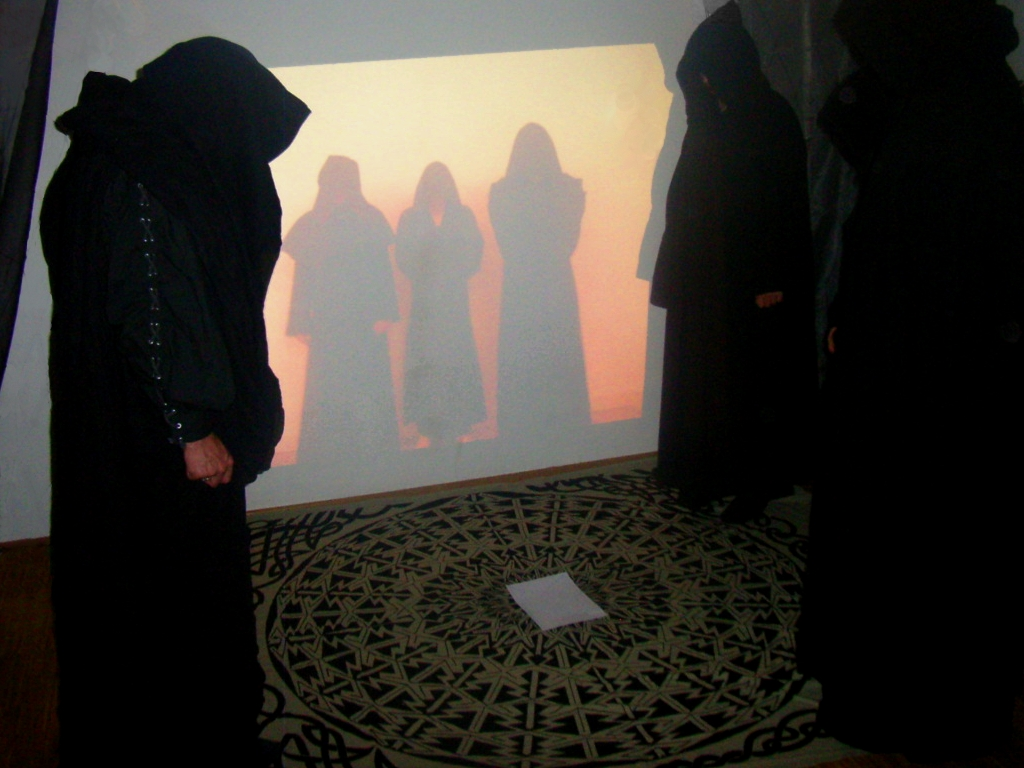
\includegraphics{videoconferencing}
    \caption{Wikimedia Commons immage `Chaos magic ritual involving videoconferencing'.}
    \label{fig:videoconf}
\end{figure}

In the image, reproduced in \Cref{fig:videoconf}\autocite{wiki:chaos}, three robed figures stand in a half-circle around a white sheet of paper placed in the centre of a circular diagram. Projected on the wall behind the chaos magi is an image of three more similarly robed figures. Based on the image's title, we can assume that these individuals are taking part in a shared ritual through videoconferencing technology.

I find both the image itself and its existence on the Wikimedia Commons extremely fascinating. Videoconferencing, both the term\footnote{Rather than, say, the hipper, more informal `video chat' or the brand names `FaceTime' or `Skype'.} and the technology itself suggest to me a mundane, boring business world of offices and meetings with remote coworkers. There is a great deal of tension between the technology and this particular use-case. That this image was captured and that the photographer chose to upload the image to Wikipedia under a Creative Commons license plays into this sense of tension between the occult underground and the business world, the ancient and the modern, the supernatural and the commonplace.

\section{Artist as Storyteller}
Write about Joshua Madara here\autocite{madara,madarabeing,madaramagic}. Maybe Mark Dion too?

% \pagebreak
% \begingroup
% \singlespacing
% \setlength{\emergencystretch}{1.5em} % this fixes overfull hboxes in citations
%                                    % (according to the interwebs)
% \printbibliography
% \endgroup
\printbibliography
\end{document}
